\documentclass[12pt, a4paper]{article}
\usepackage[utf8]{inputenc}
\usepackage{pgfplots}
\usepackage{helvet}
\usepackage{subfigure}
\usetikzlibrary{external}
\pgfplotsset{compat=1.9}
\usepgfplotslibrary{colorbrewer}
\usepgfplotslibrary{statistics}

\pgfplotsset{
    myplotstyle/.style={
    legend style={draw=none, font=\tiny},
    legend cell align=left,
    legend pos=south east,
    ylabel style={align=center, font=\sffamily\boldmath},
    xlabel style={align=center, font=\sffamily\boldmath},
    x tick label style={font=\sffamily\boldmath, align=center},
    y tick label style={font=\sffamily\boldmath, align=center},
    scaled ticks=false,
    every axis plot/.append style={thick},
    },
}
\tikzexternalize
\begin{document}
\begin{tikzpicture}
\begin{axis}[
    cycle list/Dark2,
    myplotstyle,
    table/col sep=comma,
    ylabel={Total inundation ($km^2$)},
    xlabel={Total breach area ($km^2$)}]
    \addplot+[only marks]table[x=total_breach_area, y=diff_no_breach, col sep=comma]{data/width_wet_cells.csv};
    \addlegendentry{Vary width simulations}
    \addplot+[only marks] table[x=total_breach_area, y=diff_no_breach, col sep=comma]{data/depth_wet_cells.csv};
    \addlegendentry{Vary depth simulations}
    \addplot+[only marks] table[x=total_breach_area,  y=diff_no_breach, col sep=comma]{data/width_depth_wet_cells.csv};
    \addlegendentry{Vary width and depth simulations}
\end{axis}
\end{tikzpicture}

\begin{figure}[ht]
\subfigure[]
{
\begin{tikzpicture}[scale=0.75]
    \begin{axis}
        [cycle list/Dark2,
        myplotstyle,
        table/col sep=comma,
        ylabel={Inundation area ($km^2$) \\ changes from no breach},
        xlabel={Total breach area ($km^2$)},
        legend entries={100-294 breaches, 51-100 breaches, 21-50 breaches, 16-20 breaches, 11-15 breaches,7-10 breaches, 6 breaches, 5 breach, 4 breaches, 3 breaches, 2 breaches, 1 breach},
        xtick={0,0.01,..., 0.1},
        xticklabels={},
        extra x ticks={0, 0.02,0.04, 0.06, 0.08, 0.1},
        extra x tick labels={$0$,$0.02$,  $0.04$, $0.06$,  $0.08$,  $0.1$},
        legend style={at={(.95,.05)},
                        nodes={scale=0.35, transform shape},                    
                        anchor=south east,                       
                        draw=black,                      
                        fill=white,                      
                        font=\footnotesize,                      
                        cells={anchor=west},                      
                        rounded corners=2pt,
                               }]
        \foreach \i in {100-294, 51-100, 21-50, 16-20, 11-15, 7-10, 6, 5, 4, 3, 2, 1}{
            \addplot+[only marks, draw=black, line width=.01mm]table[x=breach_area, y=inundation, col sep=comma]{../data/\i_surge.csv};
            }
    \end{axis}
\end{tikzpicture}
}
\hspace{.5cm}
\subfigure[]
{
\begin{tikzpicture}[scale=0.75]
    \begin{axis}
        [cycle list/Dark2,       
         myplotstyle,        
         table/col sep=comma,        
        %  ylabel={Inundation area ($km^2$) \\ changes from no breach},        
         xlabel={Total breach area ($km^2$)},  
         legend entries={100-294 breaches, 51-100 breaches, 21-50 breaches, 16-20 breaches, 11-15 breaches,7-10 breaches, 6 breaches, 5 breach, 4 breaches, 3 breaches, 2 breaches, 1 breach},    
         xtick={0,0.00075,0.0015,...,0.075},
         xtick distance={0.00075},        
         xticklabels={},        
         xmin=0,
         xmax=0.0075,
         ymin=0,
         ymax=25,
         extra x ticks={0, 0.0015,0.0045,0.0075},
         extra x tick labels={$0$,$0.0015$, $0.0045$, $0.0075$},      
         legend columns=1,        
         legend style={at={(.95,.05)},
                        nodes={scale=0.35, transform shape},                    
                        anchor=south east,                       
                        draw=black,                      
                        fill=white,                      
                        font=\footnotesize,                      
                        cells={anchor=west},                      
                        rounded corners=2pt,
                               }]
        
        \foreach \i in {100-294, 51-100, 21-50, 16-20, 11-15, 7-10, 6, 5, 4, 3, 2, 1}{
        \addplot+[only marks, draw=black, line width=.01mm]table[x=breach_area, y=inundation, col sep=comma]{../data/\i_surge.csv};
        }

    \end{axis}
\end{tikzpicture}}
\end{figure}


\begin{figure}
\subfigure[]
    {
    \begin{tikzpicture}[scale=0.95]
        \begin{axis}
            [cycle list/Dark2,
            myplotstyle,
            table/col sep=comma,
            ylabel={Inundation area ($km^2$) \\ changes from no breach},
            xlabel={Total breach area ($km^2$)},
            legend entries={100-294 breaches, 51-100 breaches, 21-50 breaches, 16-20 breaches, 11-15 breaches,7-10 breaches, 6 breaches, 5 breach, 4 breaches, 3 breaches, 2 breaches, 1 breach},
            xtick={0,0.01,..., 0.1},
            xticklabels={},
            extra x ticks={0, 0.02,0.04, 0.06, 0.08, 0.1},
            extra x tick labels={$0$,$0.02$,  $0.04$, $0.06$,  $0.08$,  $0.1$},
            legend style={at={(.95,.05)},
                            nodes={scale=0.35, transform shape},                    
                            anchor=south east,                       
                            draw=black,                      
                            fill=white,                      
                            font=\footnotesize,                      
                            cells={anchor=west},                      
                            rounded corners=2pt,
                                   }]
            \foreach \i in {100-294, 51-100, 21-50, 16-20, 11-15, 7-10, 6, 5, 4, 3, 2, 1}{
                \addplot+[only marks, draw=black, line width=.01mm]table[x=breach_area, y=inundation, col sep=comma]{data/\i_surge.csv};
                }
        \end{axis}

\end{tikzpicture}
}
\end{figure}

\begin{figure}
    \centering
    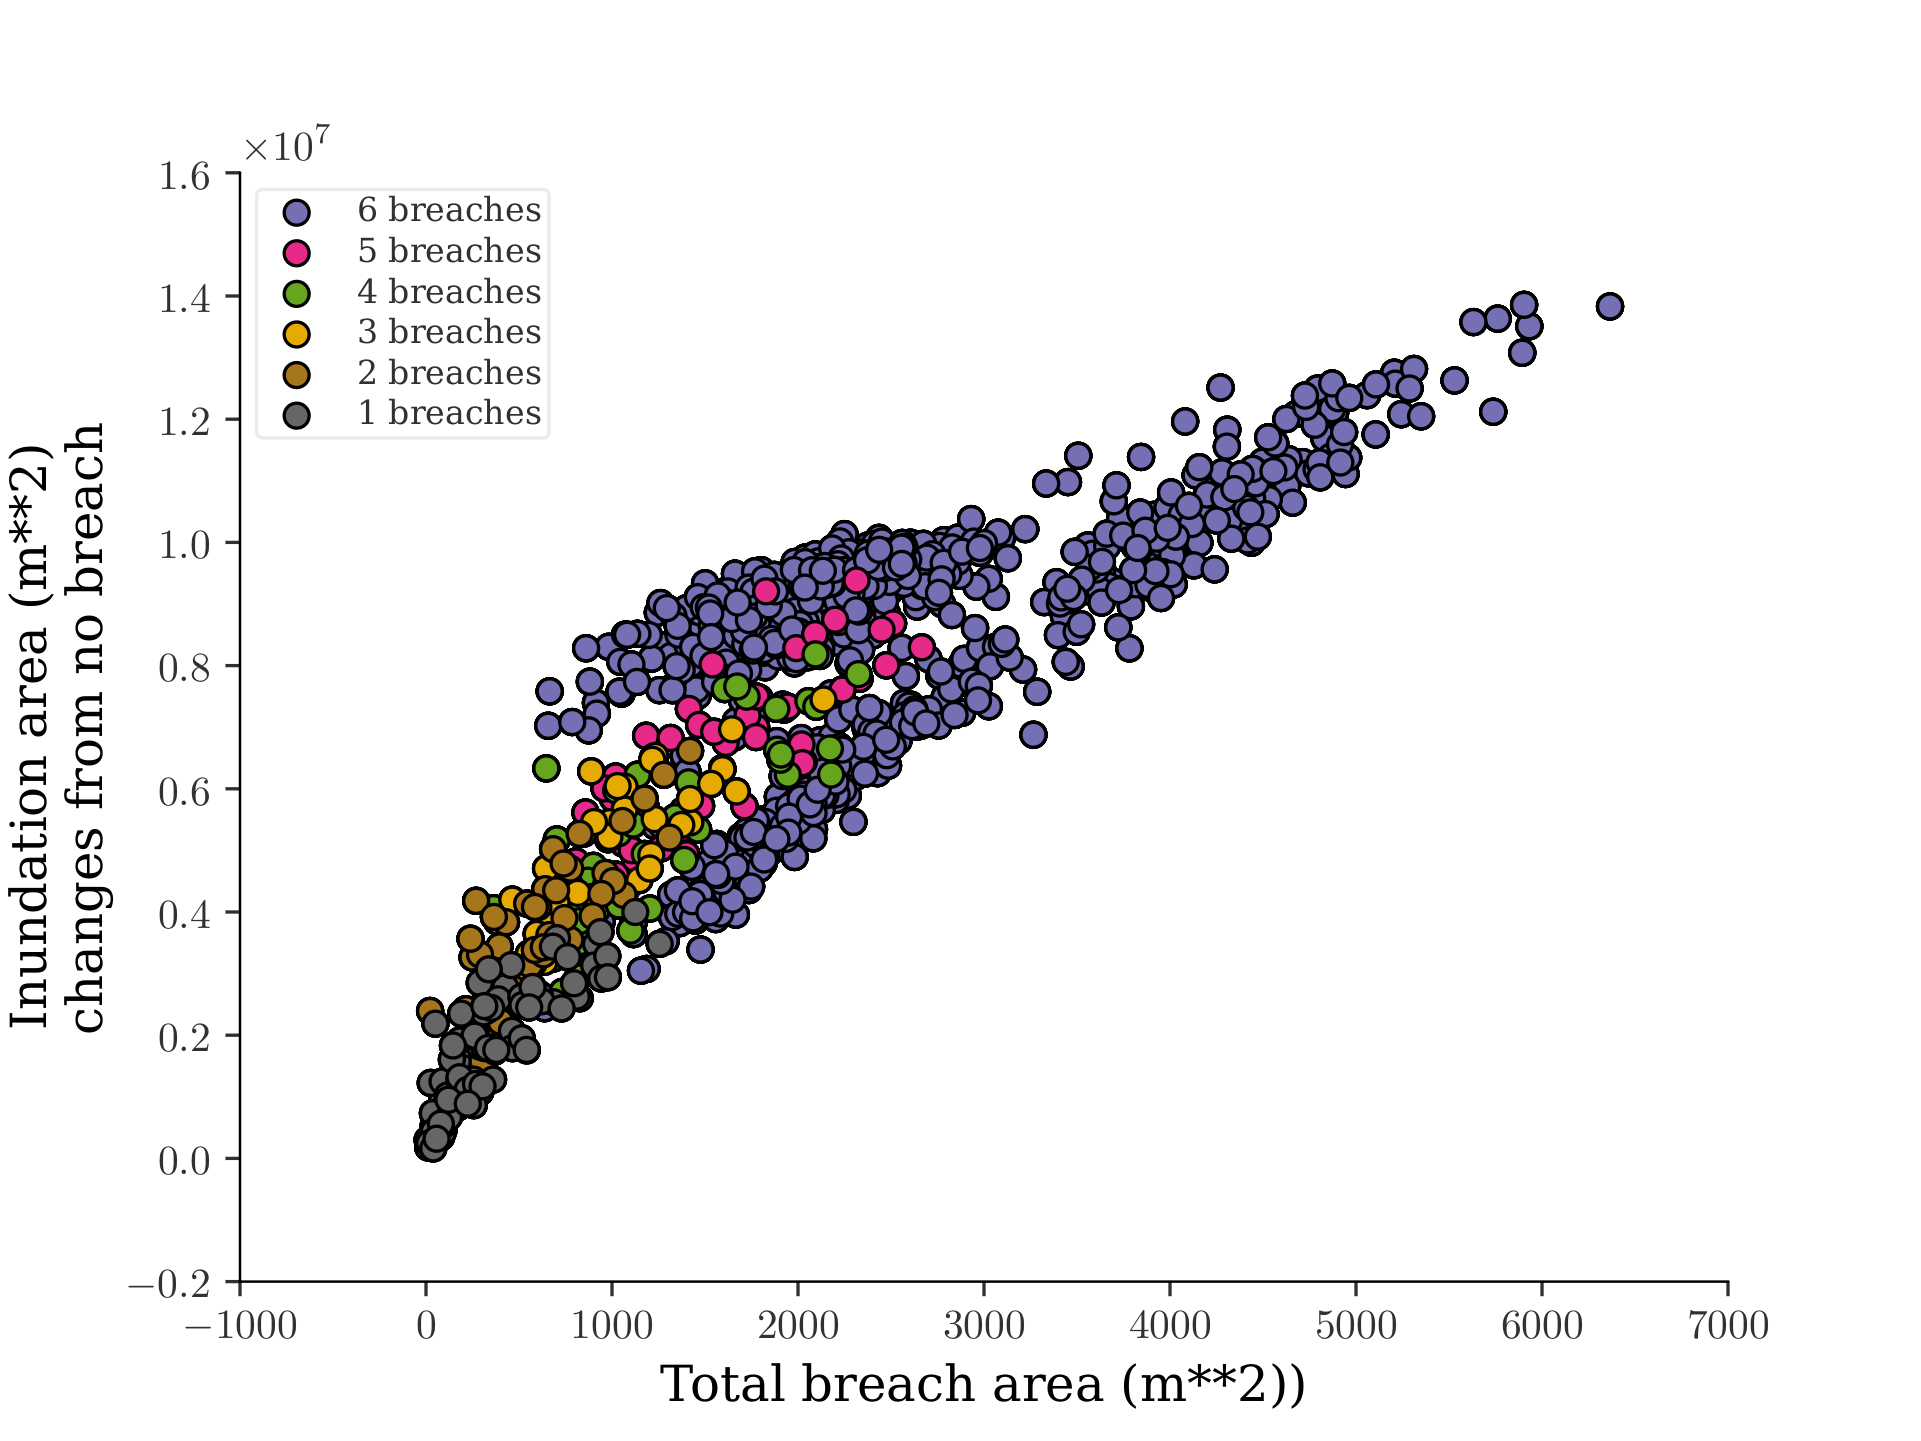
\includegraphics[width=0.75\textwidth]{inundation_x_total_breach_area.png}
    \caption{Scatter plot showing total breach area in square kilometers vs. inundation in square kilometers difference from a no breach simulation}
    \hspace{.5cm}
    \subfigure[]
    {
    \begin{tikzpicture}[scale=0.95]
        \begin{axis}
            [cycle list/Dark2,       
             myplotstyle,        
             table/col sep=comma,        
            %  ylabel={Inundation area ($km^2$) \\ changes from no breach},        
             xlabel={Total breach area ($km^2$)},  
             legend entries={100-294 breaches, 51-100 breaches, 21-50 breaches, 16-20 breaches, 11-15 breaches,7-10 breaches, 6 breaches, 5 breach, 4 breaches, 3 breaches, 2 breaches, 1 breach},    
             xtick={0,0.00075,0.0015,...,0.075},
             xtick distance={0.00075},        
             xticklabels={},        
             xmin=0,
             xmax=0.0075,
             ymin=0,
             ymax=25,
             extra x ticks={0, 0.0015,0.0045,0.0075},
             extra x tick labels={$0$,$0.0015$, $0.0045$, $0.0075$},      
             legend columns=1,        
             legend style={at={(.95,.05)},
                            nodes={scale=0.35, transform shape},                    
                            anchor=south east,                       
                            draw=black,                      
                            fill=white,                      
                            font=\footnotesize,                      
                            cells={anchor=west},                      
                            rounded corners=2pt,
                                   }]
            
            \foreach \i in {100-294, 51-100, 21-50, 16-20, 11-15, 7-10, 6, 5, 4, 3, 2, 1}{
            \addplot+[only marks, draw=black, line width=.01mm]table[x=breach_area, y=inundation, col sep=comma]{data/\i_surge.csv};
            }
    
        \end{axis}
    \end{tikzpicture}}
\end{figure}



\end{document}
